\documentclass[12pt]{article}
\usepackage{Style-Thesis-Report}

% You can define your own commands like this
\newcommand{\um}{$\upmu$m} % easily creates the label for ``micrometers''
\newcommand{\residualpanel}[1]{%
	\begin{minipage}[c][0.215\textheight][c]{0.49\textwidth}
		\centering
		\includegraphics[width=\linewidth,height=0.21\textheight,keepaspectratio]{figures/all_figures_with_residuals/#1.png}
	\end{minipage}%
}





\begin{document}
	
\begin{titlepage}
	\begin{center}
		
		\vspace*{1cm}
		
		\Huge
		\textbf{Determining the Crystaline Structure of Metals through X-Ray Diffraction}
		\large
		\vspace{1.5cm}
		
        Shukri Alex, Weltz Michael
		
		McGill University Department of Physics
		
		Supervisor: Prof. David Cooke
		
		\today
		
	\end{center}
	
\end{titlepage}

\begin{abstract}


% double paranthesis means not sure if should add

X-ray diffraction patterns were measured with a pre-calibrated Siemens D5000 diffractometer to determine the crystal structures
and lattice parameters of Cu, Ni, CuNi alloys, Sn, Pb, PbSn alloys, and two mystery samples. Peak positions were converted to
interplanar spacings using Bragg's law and indexed using candidate lattice structures and their reflection rules. Cu, Ni, and the
CuNi alloys were identified as face-centered cubic (FCC). Their experimental lattice parameters were $a_{\mathrm{Ni}}=3.5223\pm0.0001$\,\AA,
$a_{\mathrm{Cu}}=3.6126\pm0.0001$\,\AA, $a_{\mathrm{Cu_{25}Ni_{75}}}=3.5415\pm0.0002$\,\AA, $a_{\mathrm{Cu_{50}Ni_{50}}}=3.5629\pm0.0003$\,\AA,
and $a_{\mathrm{Cu_{75}Ni_{25}}}=3.5864\pm0.0002$\,\AA. Pb was also indexed as FCC, with $a_{\mathrm{Pb}}=4.94343\pm0.0001$\,\AA, while Sn was
identified as body-centered tetragonal, with $a_{\mathrm{Sn}}=5.8278\pm0.0010$\,\AA\ and $c_{\mathrm{Sn}}=3.1817\pm0.0008$\,\AA. Mystery samples
A and B were assigned FCC and primitive cubic structures, with $a_A=3.6110\pm0.0001$\,\AA\ and $a_B=3.7482\pm0.0004$\,\AA, respectively.
Lattice parameters were not determined for the Pb--Sn alloys.



%Any crystalline solid consists of a regular 3-dimensional packing of cells, the shape of 
%which corresponds to one of fourteen Bravais lattices. These 3D patterns create multiple 
%parallel planar layers within the crystal of various orientations.
%X-Rays travelling through these planes will diffract off the atoms and constructively 
%interfere at the detector, creating a peak in photon count in the observed diffraction pattern. 
%%From that peak, Bragg's law $n\lambda = 2d \sin \theta$ (where $n=1$ for a first-order plane) can be used to 
%deduce the inter-planar distance $d$ of the diffraction plane of the crystal. Using this 
%inter-planar distance and the corresponding Miller indices, the Bravais lattice can be determined
%%and the lattice parameter(s) calculated. The Cu and Ni pure samples and alloys were found to have a Face-Centered Cubic (FCC) Bravais 
%lattice, with single lattice parameters [ ... ] respectively. The alloy samples of these two 
%was found to have [ ... ]. The Sn and Pb samples were found to have a lattice of [...] 
%and parameters [...] respectively, and their alloy [...], [...]. Finally, the mystery 
%samples A and B were determined to be [...] and [...], with lattices [...] and parameters
%[...], respectively. 


\end{abstract}

\newpage

\tableofcontents{}

\thispagestyle{empty}
\pagebreak
\setcounter{page}{1}


\section{Introduction}\label{sec:int}

A solid can serve as a diffraction grating for X-rays of wavelengths similar 
to the lengths of inter-atomic distances. Similarly to how light diffracts, X-rays 
can also diffract off of atoms. Atoms within solids will arrange themselves in 
symmetries, formally called cells, given
by one of one of fourteen Bravais lattices, with each lattice grouped into one 
of seven crystal systems. These Bravais lattices govern along which diffraction
planes atoms may align and Miller indices are conventially used to index the various 
planes. Appendix \ref{A:brav} shows the different Bravais lattices.
If an X-ray is sent to a solid with an angle $\theta$ such that
constructive interference occurs at a detector placed $2\theta$ with respect to the 
incident ray, a peak in intensity of photons may be observed. From this, one can
obtain a relation between the inter-planar
distance $d$, the incident angle $\theta$, and the wavelength $\lambda$.

\begin{equation}\label{eq:brag}
	n\lambda=2d\sin(\theta)
\end{equation}
with $n=1$ for our purposes. Equation \ref{eq:brag} is formally called Bragg's Law. 

Using these observed peaks and (\ref{eq:brag}), the distance $d$ between the parallel 
diffraction planes can be obtained and related to the 
Bravais lattice and Miller indices by various equations. For a cubic system, 
this relation
takes the form of
%
\begin{equation}\label{eq:cubic}
	\frac{1}{d^2}=\frac{h^2+k^2+l^2}{a^2}
\end{equation}
%
where $h,k,l$ are the Miller Indices and $a$ is the length of the cube edge. Similar equations
for different crystal systems are given in \ref{A:brav}. Additionally, selection rules exist for each Bravais
lattice, which allow only certain diffraction planes to be observed. For instance, while any plane is allowed for a
 primitive cubic lattice, only planes with all even or all odd Miller indices are allowed for a face-centered cubic lattice.
 These selection rules are outlined for cubic and tetragonal systems in Appendix \ref{A:brav}.

\section{Methods}\label{sec:met}
% In method part, only include necessary infomation. it is not a lab manual or sop
\subsection{Instrument and Data Acquisition}
The apparatus consisted of a pre-calibrated Siemens D5000 diffractometer. 
The X-ray tube used Copper $K_{\alpha}$ radiation. 
Two sets of filters of 0.6\,mm were present on the X-ray tube and the detector.
During data acquisition, the diffractometer was set to 
40\,kV and 40\,mA. 
A computer connected to the apparatus was used to specify the measurement parameters and 
obtain the data from the instrument. A picture of the instrument is shown in Figure \ref{fig:instr}

Data acquisition consisted in mounting the sample on the mounting plate, opening the parameter 
file in the computer software and executing the job. Once the job is executed, 
the detector rotates about the mouting plate to be at an angle of 
$2\theta_0=5.00^{\circ}$ with respect to the incident rays and the mounting
plate rotates about itself to make an angle of $\theta_0$. The detector and mounting plate 
rotate with angle increments
of $2\Delta\theta=0.05$ and $\Delta\theta$, respectively, with 2.00\,s at each step  
until reaching $2\theta=110.00^{\circ}$.

Measurements were taken for samples of Copper, Nickel, Tin, Lead; 25\%, 50\% and 75\% 
alloys of Copper-Nickel and Tin-lead, and two mystery samples A and B. Three trials 
were initially done for Copper and Nickel, and two trials were done for the other samples.
This is because it was found that the uncertainties associated to statistical fluctuations of two
measurements were smaller than that associated with noise in a single data plot, expressed as standard
deviation of a fitted gaussian. Therefore, taking a second trial reduced the uncertainty in the mean
value of $d$ for a given peak, but taking a third trial did not reduce it significantly.

\begin{figure}[H]
	\centering
	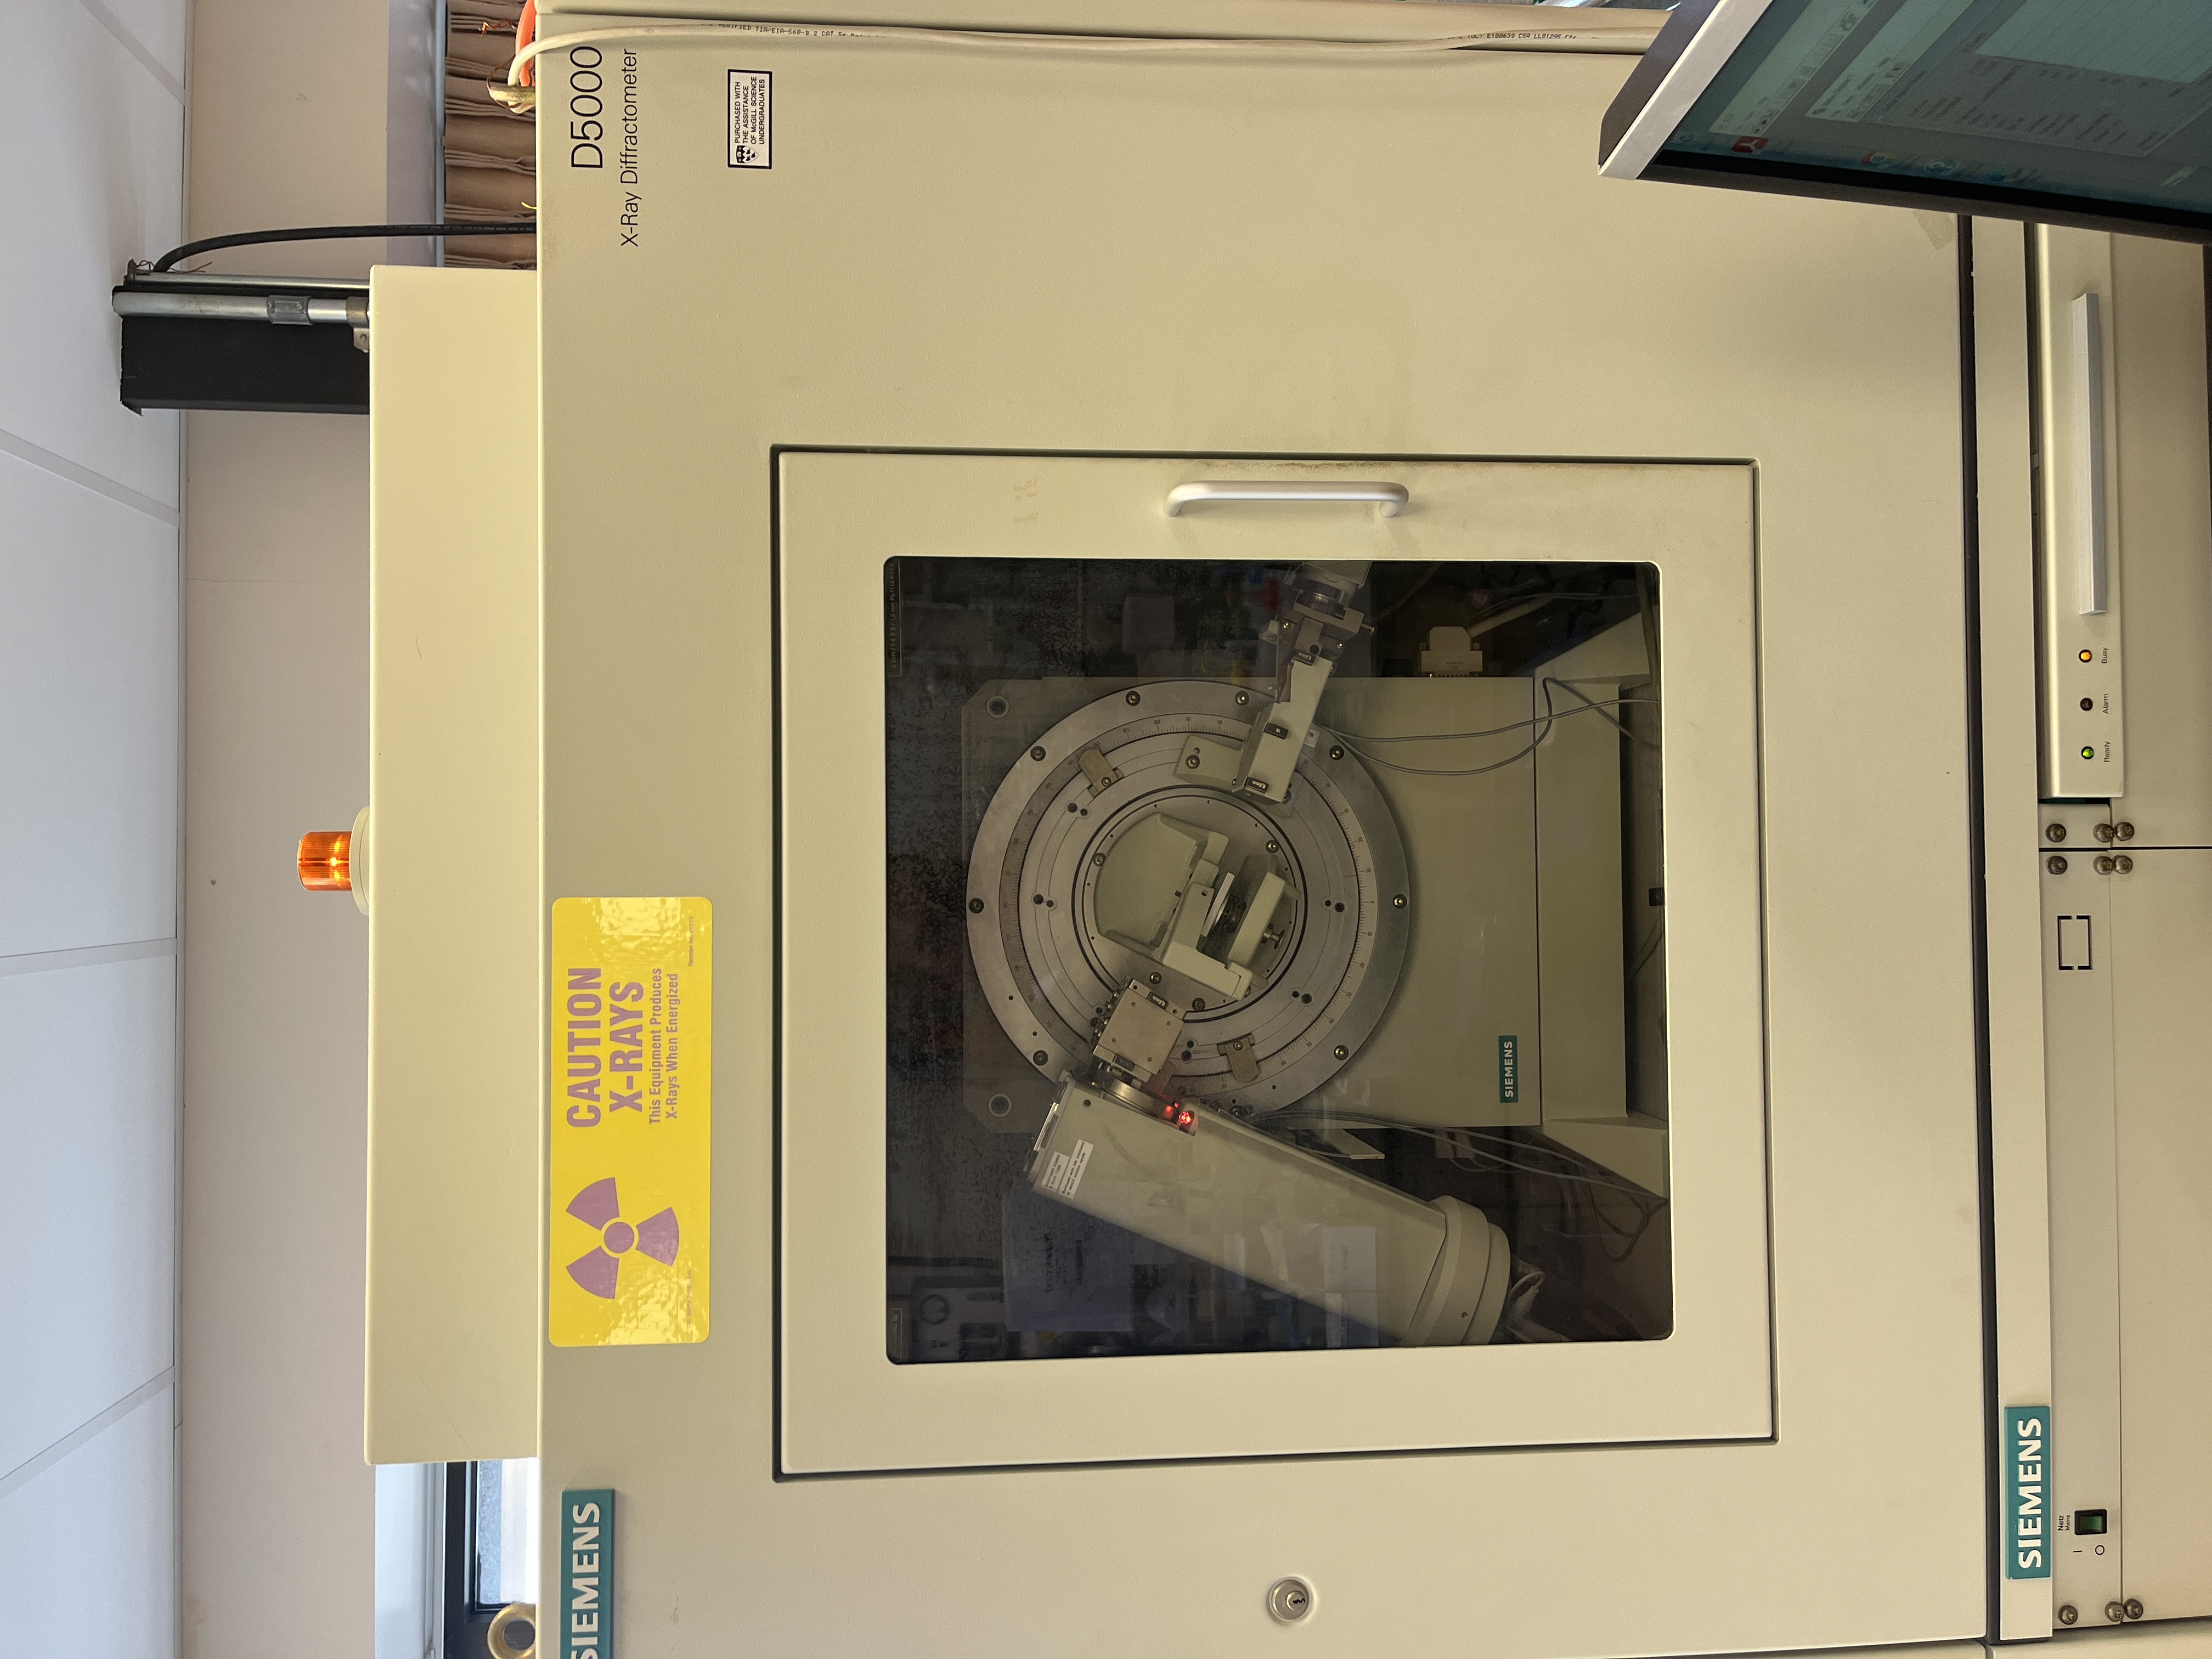
\includegraphics[width=0.4\linewidth]{figures/Instr_1.JPG}
	\caption{Picture of the Siemens D5000 diffractometer used for the experiment.}
	\label{fig:instr}
\end{figure}

% --- add picture of diffractometer --- %

% ---- 
\subsection{Data Analysis}
\label{subsec:6.1}
The measured intensity was read as a function of $2\theta$ for each sample. Candidate diffraction
peaks were identified from a smoothed intensity trace using a local-maximum
prominence threshold. These parameters were varied from sample to sample based on the characteristics
of the diffraction patterns. Smoothing was used only
for candidate detection; the peak fit used the original measured intensities.

All candidate peaks in a sample plot were fitted simultaneously with a sum of Gaussian functions and
a linear background (meant to account for a baseline count), $I_{\mathrm{fit}}(2\theta)=m(2\theta)+b+
\sum_i A_i\exp[-(2\theta-\mu_i)^2/(2\sigma_i^2)]$. The initial peak centers were the
detected positions, and the fit constrained each center to within $1^\circ$ of its initial
position and each Gaussian width to between $0.01^\circ$ and $1^\circ$. Nonlinear least
squares was performed with each count weighted by its Poisson uncertainty,
$\sqrt{\max(I,1)}$. The fitted center $\mu_i$ gives the peak position $2\theta_i$; its
uncertainty was obtained from the corresponding $\sigma_i$ standard deviation. Fit residuals
and reduced $\chi^2$ were also calculated to assess the fit.

For each fitted peak, the interplanar spacing was calculated from Bragg's law
(equation \ref{eq:brag}) using first-order diffraction and
$\lambda=1.5406\,\text{\AA}$ for a $K_\alpha$ source. The uncertainty in $d$ was propagated from the fitted
uncertainty in $2\theta$. Given that multiple plots were available per sample, weighted means and uncertainties were
calculated separately for each peak position and spacing. The values of $1/d^2$ and their
propagated uncertainties were then calculated, and ratios (often relative to the first peak, as was the case with all cubics) were
compared with the expected sequences for candidate crystal systems and Miller indices.
Candidate indices and lattice parameters were assessed for consistency with the measured
spacings; Bravais-lattice selection rules (Appendix \ref{A:brav}) were used to assess which
reflections are allowed.





\section{Results}\label{sec:res}
% Multi-panel figure is not up to expectation. All text in the figures should be 
%readable, titles are unclear, caption doesnt provide enough information, like a 
%brief information on how to interpret thr  plots and relevant statistical details. 
%more importantly, use figures to help with the flow/story telling of your paper, not 
%just a collection of all your data. Consider adding a representational xrd 
%pattern/spectrum.
%did you take any action to remove/reduce the background noise? if yes, add it into the 
%method part (and with some explanations), if not, think about what could be the 
%possible sources of background noise, and how can you reduce/remove it. 
%Three trials were done for Ni and Cu samples, though the data for the first 
%Cu trial did not save correctly. 
%For each of the alloys (including different percentage of mixing) 
%one trial was done. 

% Figure we need : sample diffraction plot, 'd' plot, sample table of 2\theta | d | 1/d^2 | hkl | miller index 

\subsection{Analysis of Copper, Nickel, and alloys}

Figure \ref{fig:cu_diff} shows the summed gaussians fitted to the diffraction pattern for a Cu sample as an example.
All other such fits are available in \ref{A:residuals}.
A $\chi^2$ value of 2.477 was obtained, showing that the results are statistically probable and 
reproducible.
From the means of the gaussians and Bragg's law the inter-planar distances were found, and then averaged for all
Cu sample runs. Angles for this particular run are shown in Table \ref{tab:cu_d}, along with the associated \underline{mean}
inter-planar distances for Cu. Uncertainties were calculated as explain in \ref{subsec:6.1}.
We first try cubic systems, so a guess is made that the first peak occurs at (100), thus $1/d^2=1/a^2$. Dividing
$1/d^2$ by $1/a^2$ for every $d$ does not yield integers. However we find that it is an integer times a 
factor of three. Hence we multiply by three and find integers for $h^2+k^2+l^2$. From these 
integer we infer $h,k,l$, and hence the Miller index for each plane. Table \ref{tab:cu_miller} show the 
values obtained following this procedure.

\begin{figure}[H]
	\centering
	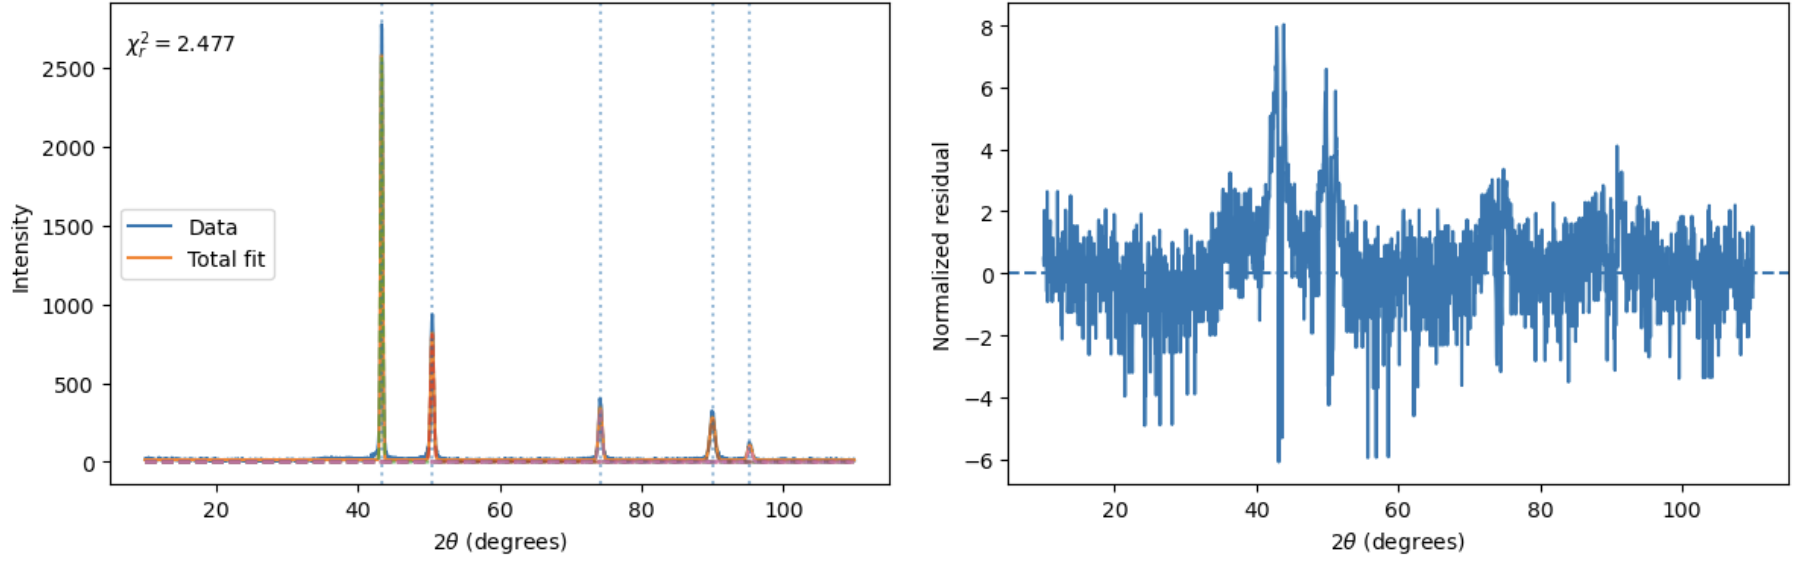
\includegraphics[width=1\linewidth]{figures/cu_diff.png}
	\caption{Plot of intensity against $2\theta$ for the Copper sample.the summed gaussians (orange) 
	are fitted to the data (blue). } 
	\label{fig:cu_diff}
\end{figure}

\begin{table}[H]
\centering
\begin{tabular}{cc}
\hline
\hline
$2\theta$ (deg) & $d_{mean}$ (\AA) \\
\hline
$43.3664 \pm 8\cdot 10^{-4}$ & $2.08485 \pm 4\cdot 10^{-5}$ \\
$50.489 \pm 2\cdot 10^{-3}$ & $1.80619 \pm 6\cdot 10^{-5}$ \\
$74.205 \pm 3\cdot 10^{-3}$ & $1.27694 \pm 5\cdot 10^{-5}$ \\
$90.017 \pm 4\cdot 10^{-3}$ & $1.08921 \pm 4\cdot 10^{-5}$ \\
$95.263 \pm 7\cdot 10^{-3}$ & $1.04260 \pm 6\cdot 10^{-5}$ \\
\hline
\hline
\end{tabular}
\caption{Angle of the peaks and the associated inter-planar distances}
\label{tab:cu_d}
\end{table}

\begin{table}[H]
\centering
\begin{tabular}{cccc}
\hline
\hline
$1/d^2$ (\AA$^{-2}$) & $\frac{1/d^2}{a^2} \cdot 3$ & $h^2+k^2+l^2$ & index\\
\hline
$0.230064 \pm 8\cdot 10^{-6}$ & $3.00 \pm 0.00$ & 3 & (111)\\
$0.30653 \pm 2\cdot 10^{-5}$ & $3.9971 \pm 3\cdot 10^{-4}$ & 4 & (200)\\
$0.61329 \pm 4\cdot 10^{-5}$ & $7.9971 \pm 6\cdot 10^{-4}$ & 8 & (220)\\
$0.84291 \pm 6\cdot 10^{-5}$ & $10.9913 \pm 8\cdot 10^{-4}$ & 11 & (311)\\
$0.9200 \pm 1\cdot 10^{-4}$ & $11.996 \pm 1\cdot 10^{-3}$ & 12 & (222)\\
\hline
\hline
\end{tabular}
\caption{Values obtained when attempting to index the Miller indices.}
\label{tab:cu_miller}
\end{table}

Based on the selection rules for cubic systems, we find that Copper is a face 
centered cubic (FCC). A similar method was applied to determine the same for Nickel, and all alloys of the two materials.
The lattice parameters were then calculated and are shown in table \ref{tab:CuNi_lattice_parameters} below, compared with
theoretical values.

\begin{table}[H]
\centering
\begin{tabular}{lccc}
\hline
\hline
Sample & $a_{\mathrm{exp}}$ (\AA) & $a_{\mathrm{theory}}$ (\AA) & $\Delta a$ (\AA) \\
\hline
Ni & $3.5223 \pm 0.0001$ & $3.5238$ & $-0.0015 \pm 0.0001$ \\
Cu & $3.6126 \pm 0.0001$ & $3.6149$ & $-0.0023 \pm 0.0001$ \\
Cu$_{25}$Ni$_{75}$ & $3.5415 \pm 0.0002$ & $3.5467$ & $-0.0052 \pm 0.0002$ \\
Cu$_{50}$Ni$_{50}$ & $3.5629 \pm 0.0003$ & $3.5696$ & $-0.0067 \pm 0.0003$ \\
Cu$_{75}$Ni$_{25}$ & $3.5864 \pm 0.0002$ & $3.5924$ & $-0.0060 \pm 0.0002$ \\
\hline
\hline
\end{tabular}
\caption{Experimental and theoretical lattice parameters for Cu, Ni pure samples and alloys. The theoretical values for the alloys are calculated using Vegard's law	.}
\label{tab:CuNi_lattice_parameters}
\end{table}

\begin{figure}[H]
	\centering
	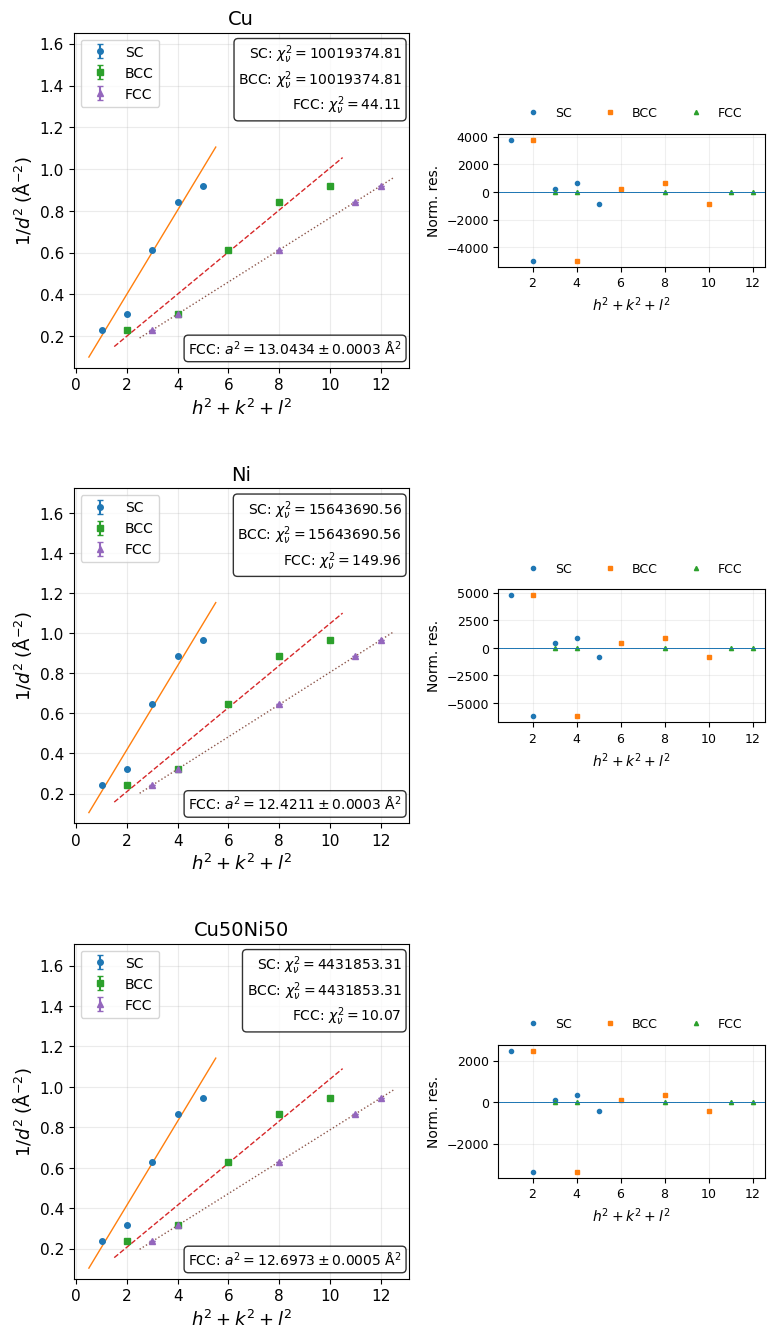
\includegraphics[width=0.8\linewidth]{figures/cubic_lattice_and_parameter_fit_Cu&Ni_new.png}
	\caption{Determination of Cubic crystal structure and lattice parameter for Cu and Ni.}
	\label{fig:CuNi_fitted_cubic_lattice}
\end{figure}

For cubics, a viable alternate method for comparison with expected sequences is to plot the experimental values against the expected sequence of
$(h^2+k^2+l^2)$ values for each of all 3 types of cubic Bravais lattices, which yielded the same results as indexing and comparing for
all copper and nickel samples (alloys included) Example such plots are shown
above in figure \ref{fig:CuNi_fitted_cubic_lattice} for mean values of $d^{-2}$.

\subsection{Lead, Tin, and alloys}
The lead and tin samples' analysis proved to be more challenging, as the peaks were greater in number and not as well defined. Still, proper tweaking of the  peak detection
parameters lead to fairly accurate identification of the peak angles, which were then used to calculate the interplanar distances as with Cu and Ni. Lead (Pb) followed a
pattern similar to that of Cu and Ni, though showing many more peaks; it was indexed as another face-centered cubic (FCC) system, with a lattice parameter of $a_{Pb}=4.94343\pm 0.0001$\,\AA.
As it is repetitive, the indexing of the lead sample is not shown here, but is available in the supplementary material. The tin sample required more in-depth analysis,
as it did not match any cubic crystal structure. It was eventually identified to be a body-centered tetragonal, with parameters $a_{Sn}=5.8278 \pm 0.0010$\,\AA\ and $c_{Sn}=3.1817 \pm 0.0008$\,\AA.
As for the alloys, time proved insufficient to complete that part of the analysis, and no lattice parameter values were obtained. Still, some discussion of the data will be provided. Indexing of
samples containing Sn is too bulky to be shown here, but is available in the supplementary material. Further discussion of the analysis of these samples is done
 in section \ref{sec:dis}.

\subsection{Mystery Samples A and B}
Analysis of the mystery samples provided was actually quite straightforward. Building upon the methodology developed for Copper and Nickel,
sample A was quickly found to be a cubic system with a face-centered lattice, with a ratio sequence and Miller indices identical to that of the Copper
and Nickel samples; sample B proved to be a cubic system with a primitive lattice. Again, as it is repetitive, the indexing of sample A is not shown here, but is
available in the supplementary material. The indexing of sample B is shown in table \ref{tab:B_indexing} below, where $a$ is the first interplanar distance,
as is the case with a PC.
The lattice parameters were calculated to be $a_A=3.6110\pm 0.0001$\,\AA and $a_B=3.7482\pm 0.0004$\,\AA\, respectively.

\begin{table}[H]
\centering
\begin{tabular}{c c c c}
\hline
$1/d^2$ (\AA$^{-2}$) &
$\frac{1/d^2}{a^2}$ &
Expected PC ratio &
Miller indices \\
\hline
\hline
$0.071179 \pm 0.000016$ & $1.00 \pm 0.00$ & 1  & (100) \\
$0.142535 \pm 0.000020$ & $2.00248 \pm 0.00054$ & 2  & (110) \\
$0.213807 \pm 0.000010$ & $3.00379 \pm 0.00071$ & 3  & (111) \\
$0.285031 \pm 0.000021$ & $4.00442 \pm 0.00097$ & 4  & (200) \\
$0.356334 \pm 0.000050$ & $5.0062 \pm 0.0014$ & 5  & (210) \\
$0.427618 \pm 0.000065$ & $6.0076 \pm 0.0017$ & 6  & (211) \\
$0.570263 \pm 0.000036$ & $8.0117 \pm 0.0019$ & 8  & (220) \\
$0.64134 \pm 0.00011$ & $9.0102 \pm 0.0026$ & 9  & (221), (300) \\
$0.71252 \pm 0.00016$ & $10.0103 \pm 0.0033$ & 10 & (310) \\
$0.784099 \pm 0.000050$ & $11.0159 \pm 0.0026$ & 11 & (311) \\
$0.85524 \pm 0.00011$ & $12.0153 \pm 0.0032$ & 12 & (222) \\
$0.92726 \pm 0.00026$ & $13.0271 \pm 0.0048$ & 13 & (320) \\
$0.99755 \pm 0.00018$ & $14.0146 \pm 0.0041$ & 14 & (321) \\
\hline
\end{tabular}
\caption{XRD peak indexing for sample B.}
\label{tab:B_indexing}
\end{table}

\section{Discussion}\label{sec:dis}
The CuNi samples provide the clearest test of the peak-indexing procedure. The measured Cu reflections are consistent with the sequence $(111)$, $(200)$, $(220)$, $(311)$, and $(222)$,
and satisfy the FCC selection rule that the Miller indices are either all odd or all even. The corresponding cubic fits give the same FCC sequences for Ni and for the Cu--Ni alloys. The
measured lattice parameter increases with Cu content, from $3.5223 \pm 0.0001$\,\AA\ for Ni to $3.6126 \pm 0.0001$\,\AA\ for Cu, which is in close agreement with the linear Vegard-law estimates
listed in Table \ref{tab:CuNi_lattice_parameters}.

All five experimental lattice parameters in that table are lower than their theoretical or Vegard-law values. The differences range from $0.0015$ to $0.0067$\,\AA\ (less than $0.2\%$), but are larger
than the quoted fit-based uncertainties. This means those small uncertainties describe the precision estimated from the fitted peaks and repeat measurements rather the full accuracy of the lattice parameters,
which is a flaw in our method. The reported Cu fit statistic of $\chi^2=2.477$ should likewise be interpreted together with its degrees of freedom and the precise definition of the statistic; it does not on its
own demonstrate reproducibility, but the other Cu runs shown in the appendix, and the similarity between runs for each sample, also show in \ref{A:residuals} do. In the end, the CuNi results do show that the
combination of Bragg's law, Miller-index sequences, and lattice selection rules can identify structures and estimate lattice parameters from measured diffraction peaks, which was the primary goal of this preliminary study.

The Pb and Sn results show the importance of comparing candidate crystal systems rather than assuming that every sample is cubic. The Pb pattern was found as FCC, with $a_{\mathrm{Pb}}=4.94343 \pm 0.0001$\,\AA, while the Sn
one did not match a cubic sequence and was shown to be a body-centered tetragonal structure, with $a_{\mathrm{Sn}}=5.8278 \pm 0.0010$\,\AA\ and $c_{\mathrm{Sn}}=3.1817 \pm 0.0008$\,\AA. Indexing the Sn pattern required testing
candidate crystal systems in turn. After the ratio sequence ruled out all three cubic lattices, a body-centered tetragonal lattice was assumed, so that only reflections with $h+k+l$ even were considered. With two unknown lattice parameters,
the peak positions alone do not fix the indices, so the assignment was made by trial and error. Candidate $(hkl)$ were matched to the measured peaks starting from approximate $a$ and $c$ values, and $a$ and $c$ were then refined by a least-squares
fit of $1/d^2=(h^2+k^2)/a^2+l^2/c^2$ to all indexed peaks. The final assignment of parameters was accepted because every indexed peak fell within $0.1^{\circ}$ of its calculated position. Several reflections that satisfy $h+k+l$ even, such as
$(110)$, $(002)$ and $(310)$, never appear, which is expected since Sn crystallizes in the $I4_1/amd$ space group, which has additional extinction rules beyond those of Appendix \ref{A:brav}. The lowest-angle peak ($2\theta\approx28.5^{\circ}$)
could not be matched to any allowed Sn reflection and was discarded, likely as a contaminant.

This is also in close accordance with theoretical
values. The PbSn alloy patterns were indexed as a superposition of two separate phases, FCC Pb and body-centered tetragonal Sn, rather than as a single new structure. Most detected peaks could be assigned to one of the two phases except
for a few likely false peaks, results of the difficult fit of the obtained diffraction pattern. This is consistent with the PbSn system having very limited mutual solubility, in
contrast to the CuNi alloys, which formed a single FCC phase. Vegard's law therefore does not apply here.

The two mystery patterns were assigned to cubic structures: sample A to FCC and sample B to primitive cubic (PC), based on their observed ratio sequences and the applicable selection rules. These assignments describe
the diffraction patterns; the results presented here do not independently establish the chemical identities of the samples. However, it does strongly suggest that is the case.


\section{Conclusion}\label{sec:con}
X-ray diffraction combined with Bragg's law and Miller-index selection rules was enough to identify the crystal structure of every sample in this study, with minimal assumptions. Cu, Ni, Pb and mystery sample A were indexed as FCC,
mystery sample B as primitive cubic, and Sn as body-centered tetragonal. The CuNi alloys remained a single FCC phase, with lattice parameters that followed Vegard's law to within $0.2\%$. The PbSn alloys instead behaved as a mixture
of separate Pb and Sn phases, which reflects the limited mutual solubility of the two metals. The lattice parameters were consistently slightly below the expected values by more than their statistical uncertainties, so the quoted errors
reflect precision and not the full accuracy of the measurement. A limitation in the shown results is that the PbSn alloys were only qualitatively analyzed, without lattice parameters. Future work could use a reference standard to correct systematic
angle offsets, include a quantitative fit of the PbSn phases, and use peak intensities to estimate phase fractions.

\newpage


% Bibliography:
\bibliographystyle{IEEEtran}
\bibliography{Report template/MyBibliography}

%-----------------------------------%

\section{Appendix}
\subsection{Inter-planar distance, Bravais Lattices and Miller indices}\label{A:brav}

\begin{figure}[H]
	\centering
	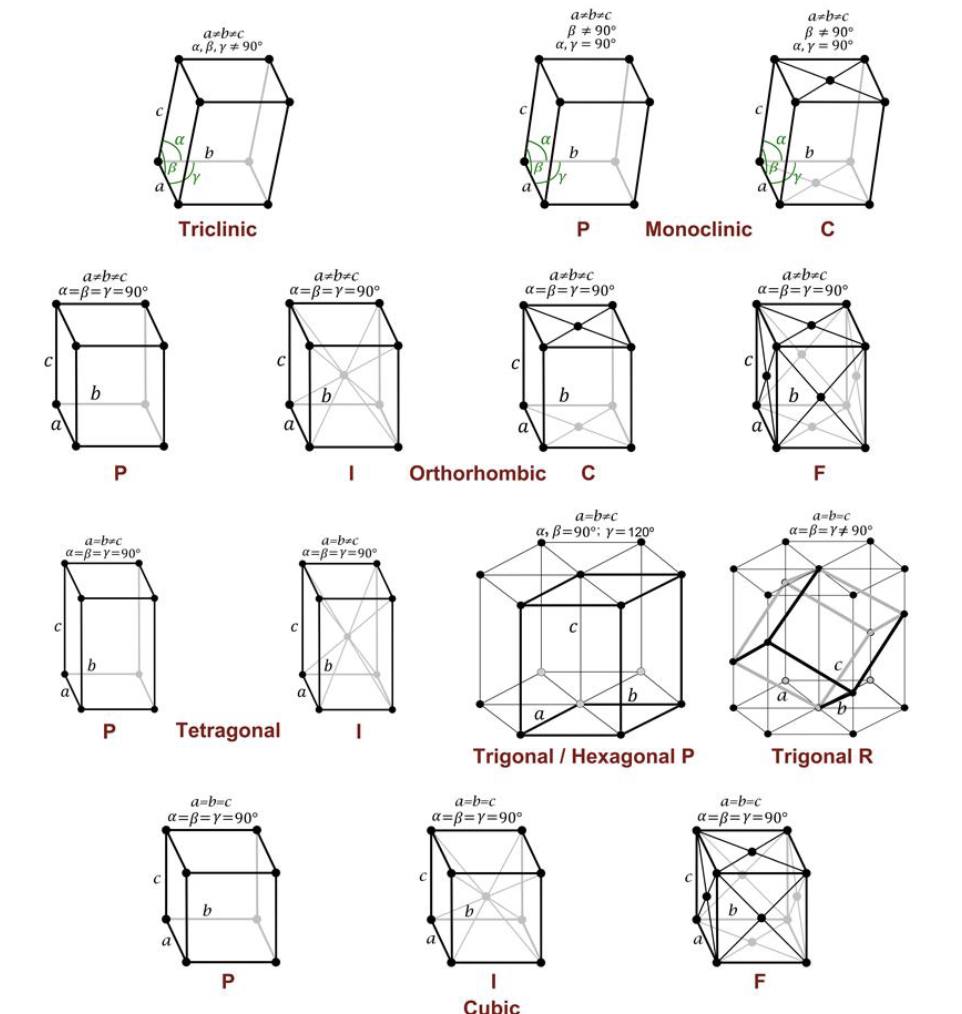
\includegraphics[width=0.4\linewidth]{figures/brav_lat.png}
	\caption{Fourteen Bravais lattices and their seven associated groups.}
\end{figure}

The selection rules for cubic systems are as follows:
\begin{itemize}
	\item PC: all $h,k,l$ allowed
	\item FCC: all even or all odd $h,k,l$ allowed
	\item BCC: $h+k+l$ even
\end{itemize}

For tetragonal systems, the selection rules are as follows:

\begin{itemize}
	\item P: all $h,k,l$ allowed
	\item I: $h+k+l$ even
\end{itemize}

\newpage

For the following equations: $d$ is the inter planar distance, $a,b,c$
the inter-atomic distances, $h,k,l$ the indices for a given Miller index (hkl).

Cubic: \[\frac{1}{d^2}=\frac{h^2+k^2+l^2}{a^2}\]

Tetragonal: \[\frac{1}{d^2}=\frac{h^2+k^2}{a^2}+\frac{l^2}{c^2}\]

Hexagonal: \[\frac{1}{d^2}=\frac{4}{3}(\frac{h^2+k^2+hk}{a^2})+\frac{l^2}{c^2}\]

Orthorhombic: \[\frac{1}{d^2}=\frac{h^2}{a^2}+\frac{k^2}{b^2}+\frac{l^2}{c^2}\]

Vegard's law: \[a_{alloy}=x a_{Cu}+(1-x) a_{Ni}\]


\clearpage
\subsection{Supplementary Indexing Tables}
\label{A:indexing-tables}
\newcommand{\indexingpanel}[2]{%
	\begin{minipage}[c][0.17\textheight][c]{0.48\textwidth}
		\centering
		\normalsize\textbf{#1}\\[0.15em]
		\includegraphics[width=\linewidth,height=0.155\textheight,keepaspectratio]{\detokenize{figures/indexing tables/#2.png}}
	\end{minipage}%
}

\noindent
\begin{tabular}{@{}c@{\hspace{0.02\textwidth}}c@{}}
	\indexingpanel{Cu$_{25}$Ni$_{75}$}{Cu25Ni75} & \indexingpanel{Cu$_{50}$Ni$_{50}$}{Cu50Ni50} \\
	\indexingpanel{Cu$_{75}$Ni$_{25}$}{Cu75Ni25} & \indexingpanel{Ni}{Ni} \\
	\indexingpanel{Sn}{Sn} & \indexingpanel{Pb$_{25}$Sn$_{75}$}{Pb25Sn75} \\
	\indexingpanel{Pb$_{50}$Sn$_{50}$}{Pb50Sn50} & \indexingpanel{Pb$_{75}$Sn$_{25}$}{Pb75Sn25} \\
	\indexingpanel{Mystery sample A}{A} & \rule{0pt}{0.17\textheight}
\end{tabular}

\clearpage
\subsection{Supplementary Gaussian Fits and Residuals}
\label{A:residuals}

\noindent\textbf{Gaussian fits and normalized residuals (1/3)}\par\vspace{0.2em}
\begin{center}
\begin{tabular}{@{}c@{\hspace{0.01\textwidth}}c@{}}
	\residualpanel{Cu\_10-09-26\_2} & \residualpanel{Ni\_08-09-26} \\
	\residualpanel{Ni\_10-09-26} & \residualpanel{Ni\_10-09-26\_2} \\
	\residualpanel{Cu25Ni75\_14-09-26} & \residualpanel{Cu25Ni75\_29-09-26} \\
	\residualpanel{Cu50Ni50\_14-09-26} & \residualpanel{Cu50Ni50\_29-09-26}
\end{tabular}
\end{center}

\newpage
\noindent\textbf{Gaussian fits and normalized residuals (2/3)}\par\vspace{0.2em}
\begin{center}
\begin{tabular}{@{}c@{\hspace{0.01\textwidth}}c@{}}
	\residualpanel{Cu75Ni25\_14-09-26} & \residualpanel{Cu75Ni25\_29-09-26} \\
	\residualpanel{Pb\_15-09-26} & \residualpanel{Pb\_24-09-26} \\
	\residualpanel{Sn\_15-09-26} & \residualpanel{Sn\_24-09-26} \\
	\residualpanel{Pb25Sn75\_05-10-26} & \residualpanel{Pb25Sn75\_15-09-26}
\end{tabular}
\end{center}

\newpage
\noindent\textbf{Gaussian fits and normalized residuals (3/3)}\par\vspace{0.2em}
\begin{center}
\begin{tabular}{@{}c@{\hspace{0.01\textwidth}}c@{}}
	\residualpanel{Pb50Sn50\_15-09-26} & \residualpanel{Pb50Sn50\_24-09-26} \\
	\residualpanel{Pb75Sn25\_02-10-26} & \residualpanel{Pb75Sn25\_15-09-26} \\
	\residualpanel{A\_17-09-26} & \residualpanel{A\_17-09-26\_2} \\
	\residualpanel{B\_17-09-26} & \residualpanel{B\_17-09-26\_2}
\end{tabular}
\end{center}

\end{document}